\documentclass[12pt,a4paper]{article}
\usepackage[utf8]{inputenc}
\usepackage[croatian]{babel}
\usepackage{geometry}
\usepackage{graphicx}
\usepackage{pgfplots}
\pgfplotsset{compat=1.18}
\usepackage{booktabs}
\usepackage{xcolor}
\usepackage{hyperref}
\usepackage{enumitem}
\usepackage{fancyhdr}
\usepackage{listings}
\usepackage{float}

\geometry{margin=2.5cm}

% Boje za ozbiljnost
\definecolor{critical}{RGB}{220, 53, 69}
\definecolor{high}{RGB}{255, 193, 7}
\definecolor{medium}{RGB}{255, 152, 0}
\definecolor{low}{RGB}{40, 167, 69}

% Header i Footer
\pagestyle{fancy}
\fancyhf{}
\fancyhead[L]{\leftmark}
\fancyhead[R]{Izvještaj o Inspekciji Koda}
\fancyfoot[C]{\thepage}
\renewcommand{\headrulewidth}{0.4pt}
\renewcommand{\footrulewidth}{0pt}

% Hyperref postavke
\hypersetup{
    colorlinks=true,
    linkcolor=blue,
    filecolor=magenta,      
    urlcolor=cyan,
    pdftitle={Izvještaj o Inspekciji Koda - RestaurantInventory},
    pdfauthor={Tim 4}
}

\title{\textbf{Izvještaj o Inspekciji Koda}\\
\large RestaurantInventory - Tim 4}
\author{}
\date{}

\begin{document}

\maketitle
\thispagestyle{empty}

\vspace{2cm}

\begin{center}
\textbf{Informacije o Inspekciji}
\end{center}

\begin{table}[H]
\centering
\begin{tabular}{ll}
\textbf{Datum inspekcije:} & 2024 \\
\textbf{Moderator inspekcije:} & [Ime Moderatora] \\
\textbf{Tim:} & Tim 4 \\
\textbf{Aplikacija:} & RestaurantInventory \\
\textbf{Verzija izvještaja:} & 1.0 \\
\end{tabular}
\end{table}

\newpage
\tableofcontents
\newpage

\section{Uvod}

Ovaj dokument predstavlja izvještaj o inspekciji koda aplikacije \textbf{RestaurantInventory}, konzolne aplikacije za upravljanje inventarom restorana. Inspekcija je provedena u sklopu laboratorijske vježbe 4, a cilj je bio identifikovati probleme u kodu, kategorizirati ih prema ozbiljnosti i izvršiti Pareto analizu uzroka i defekata.

\subsection{Pregled Aplikacije}

Aplikacija \textbf{RestaurantInventory} omogućava:
\begin{itemize}
    \item Dodavanje stavki u inventar
    \item Pretraživanje i filtriranje stavki
    \item Ažuriranje postojećih stavki
    \item Uklanjanje stavki iz inventara
    \item Generisanje izvještaja
\end{itemize}

\subsection{Statistika Koda}

\begin{table}[H]
\centering
\begin{tabular}{lr}
\toprule
\textbf{Metrika} & \textbf{Vrijednost} \\
\midrule
Ukupno linija koda & $\sim$600 \\
Broj klasa & 10 \\
Broj servisa & 4 \\
Broj modela & 6 \\
\bottomrule
\end{tabular}
\caption{Osnovne metrike koda}
\end{table}

\section{Kategorizacija Problema}

Tokom inspekcije koda, identifikovano je \textbf{15 problema} koji su kategorizirani prema ozbiljnosti:

\begin{table}[H]
\centering
\begin{tabular}{lcc}
\toprule
\textbf{Ozbiljnost} & \textbf{Broj} & \textbf{Postotak} \\
\midrule
\textcolor{critical}{Kritični (Critical)} & 3 & 20\% \\
\textcolor{high}{Visoki (High)} & 7 & 47\% \\
\textcolor{medium}{Srednji (Medium)} & 3 & 20\% \\
\textcolor{low}{Niski (Low)} & 2 & 13\% \\
\midrule
\textbf{Ukupno} & \textbf{15} & \textbf{100\%} \\
\bottomrule
\end{tabular}
\caption{Raspodjela problema po ozbiljnosti}
\end{table}

\subsection{Kritični Problemi}

\subsubsection{ISSUE-001: NullReferenceException u InventarService.DodajStavku}

\textbf{Lokacija:} \texttt{Services/InventarService.cs:22-24} \\
\textbf{Ozbiljnost:} \textcolor{critical}{Kritična} \\
\textbf{Checklist:} Validacija inputa, Null Safety

\textbf{Problem:} Ako \texttt{stavka.Dobavljac} ili postojeća stavka u listi ima \texttt{null} vrijednost za \texttt{Dobavljac}, poziv \texttt{Equals} će baciti \texttt{NullReferenceException}.

\textbf{Rješenje:} Dodati null-checking prije poziva \texttt{Equals}:

\begin{lstlisting}[language=CSharp, basicstyle=\small]
if (inventar.Stavke.Any(s => 
    string.Equals(s.Naziv, stavka.Naziv, StringComparison.OrdinalIgnoreCase) &&
    string.Equals(s.Dobavljac ?? "", stavka.Dobavljac ?? "", 
                  StringComparison.OrdinalIgnoreCase)))
\end{lstlisting}

\subsubsection{ISSUE-002: Nevalidiran unos cijene može baciti FormatException}

\textbf{Lokacija:} \texttt{Program.cs:134} \\
\textbf{Ozbiljnost:} \textcolor{critical}{Kritična} \\
\textbf{Checklist:} Error Handling

\textbf{Problem:} Ako korisnik unese nevalidan string (npr. "abc"), \texttt{double.Parse} će baciti \texttt{FormatException} koja nije uhvaćena.

\textbf{Rješenje:} Koristiti \texttt{double.TryParse} umjesto \texttt{double.Parse}.

\subsubsection{ISSUE-003: Logička greška u StavkaInventaraService.JeKriticna}

\textbf{Lokacija:} \texttt{Services/StavkaInventaraService.cs:8-24} \\
\textbf{Ozbiljnost:} \textcolor{critical}{Kritična} \\
\textbf{Checklist:} Logika aplikacije

\textbf{Problem:} Metoda \texttt{JeKriticna} ima logičku grešku. Ako je \texttt{stavka.Kolicina < stavka.MinKolicina}, metoda uvijek vraća \texttt{true} bez obzira na ostale uslove (linija 18 je unreachable code).

\textbf{Rješenje:} Refaktorisati logiku da bude jasnija i ispravna.

\subsection{Visoki Problemi}

Među visokim problemima su:
\begin{itemize}
    \item Duplikacija koda između \texttt{FilterService} i \texttt{InventarService.Pretrazi}
    \item Nedostaje validacija inputa na više mjesta
    \item Nedostaje logging mehanizam
    \item Nedostaju unit testovi
    \item Nedostaje dokumentacija
    \item Nekonzistentno imenovanje (miješanje jezika)
    \item Hardcoded vrijednosti (magic numbers)
\end{itemize}

\section{Pareto Analiza}

\subsection{Pareto Analiza po Uzrocima}

Analizom problema po uzrocima, identifikovano je nekoliko glavnih kategorija uzroka:

\begin{table}[H]
\centering
\begin{tabular}{lcc}
\toprule
\textbf{Uzrok} & \textbf{Broj Problema} & \textbf{Postotak} \\
\midrule
Nedostaje validacija & 4 & 26.7\% \\
Nedostaje dokumentacija/testiranje & 3 & 20.0\% \\
Nekonzistentnost & 3 & 20.0\% \\
Duplikacija koda & 2 & 13.3\% \\
Logičke greške & 2 & 13.3\% \\
Nedostaje infrastruktura (DI, Config) & 2 & 13.3\% \\
Stilski problemi & 2 & 13.3\% \\
\bottomrule
\end{tabular}
\caption{Analiza problema po uzrocima}
\end{table}

\begin{figure}[H]
\centering
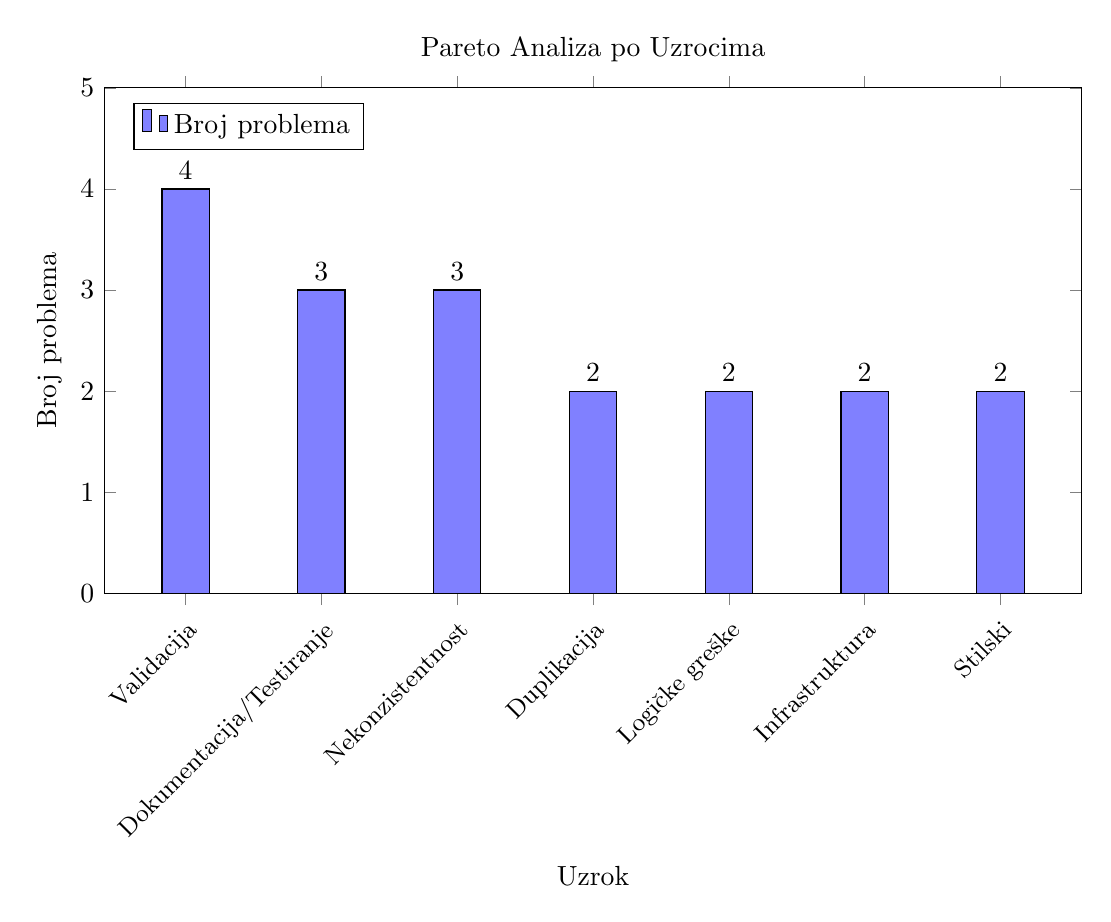
\begin{tikzpicture}
\begin{axis}[
    ybar,
    bar width=0.6cm,
    width=14cm,
    height=8cm,
    ylabel={Broj problema},
    xlabel={Uzrok},
    symbolic x coords={Validacija, Dokumentacija/Testiranje, Nekonzistentnost, Duplikacija, Logičke greške, Infrastruktura, Stilski},
    xtick=data,
    xticklabel style={rotate=45, anchor=north east, font=\small},
    ymin=0,
    ymax=5,
    legend pos=north west,
    title={Pareto Analiza po Uzrocima},
    nodes near coords,
    nodes near coords align={vertical},
]
\addplot[fill=blue!50] coordinates {
    (Validacija, 4)
    (Dokumentacija/Testiranje, 3)
    (Nekonzistentnost, 3)
    (Duplikacija, 2)
    (Logičke greške, 2)
    (Infrastruktura, 2)
    (Stilski, 2)
};
\legend{Broj problema}
\end{axis}
\end{tikzpicture}
\caption{Pareto dijagram - Analiza po uzrocima (sortirano po broju problema)}
\end{figure}

\begin{table}[H]
\centering
\begin{tabular}{lcc}
\toprule
\textbf{Uzrok} & \textbf{Broj} & \textbf{Kumulativni postotak} \\
\midrule
Validacija & 4 & 22.2\% \\
Dokumentacija/Testiranje & 3 & 38.9\% \\
Nekonzistentnost & 3 & 55.6\% \\
Duplikacija & 2 & 66.7\% \\
Logičke greške & 2 & 77.8\% \\
Infrastruktura & 2 & 88.9\% \\
Stilski & 2 & 100.0\% \\
\bottomrule
\end{tabular}
\caption{Kumulativna analiza po uzrocima}
\end{table}

\textbf{80/20 Pravilo:}

Top 3 uzroka (Validacija, Dokumentacija/Testiranje, Nekonzistentnost) čine \textbf{55.6\%} svih problema. Top 4 uzroka čine \textbf{66.7\%} svih problema, što je blizu 80/20 principa. Fokusiranje na ove kategorije bi riješilo većinu problema.

\subsection{Pareto Analiza po Defektima}

Analizom problema po tipovima defekata i njihovoj ozbiljnosti:

\begin{table}[H]
\centering
\begin{tabular}{lccc}
\toprule
\textbf{Tip Defekta} & \textbf{Broj} & \textbf{Ozbiljnost} & \textbf{Prioritet} \\
\midrule
NullReferenceException rizici & 2 & \textcolor{critical}{Kritična} & P1 \\
FormatException rizici & 1 & \textcolor{critical}{Kritična} & P1 \\
Logičke greške & 1 & \textcolor{critical}{Kritična} & P1 \\
Duplikacija koda & 1 & \textcolor{high}{Visoka} & P2 \\
Nedostaje validacija & 4 & \textcolor{high}{Visoka} & P2 \\
Nedostaje logging & 1 & \textcolor{high}{Visoka} & P2 \\
Nedostaju testovi & 1 & \textcolor{high}{Visoka} & P2 \\
Nedostaje dokumentacija & 1 & \textcolor{high}{Visoka} & P2 \\
Arhitektonski problemi & 2 & \textcolor{medium}{Srednja} & P3 \\
Stilski problemi & 3 & \textcolor{low}{Niska} & P4 \\
\bottomrule
\end{tabular}
\caption{Analiza problema po tipovima defekata}
\end{table}

\begin{figure}[H]
\centering
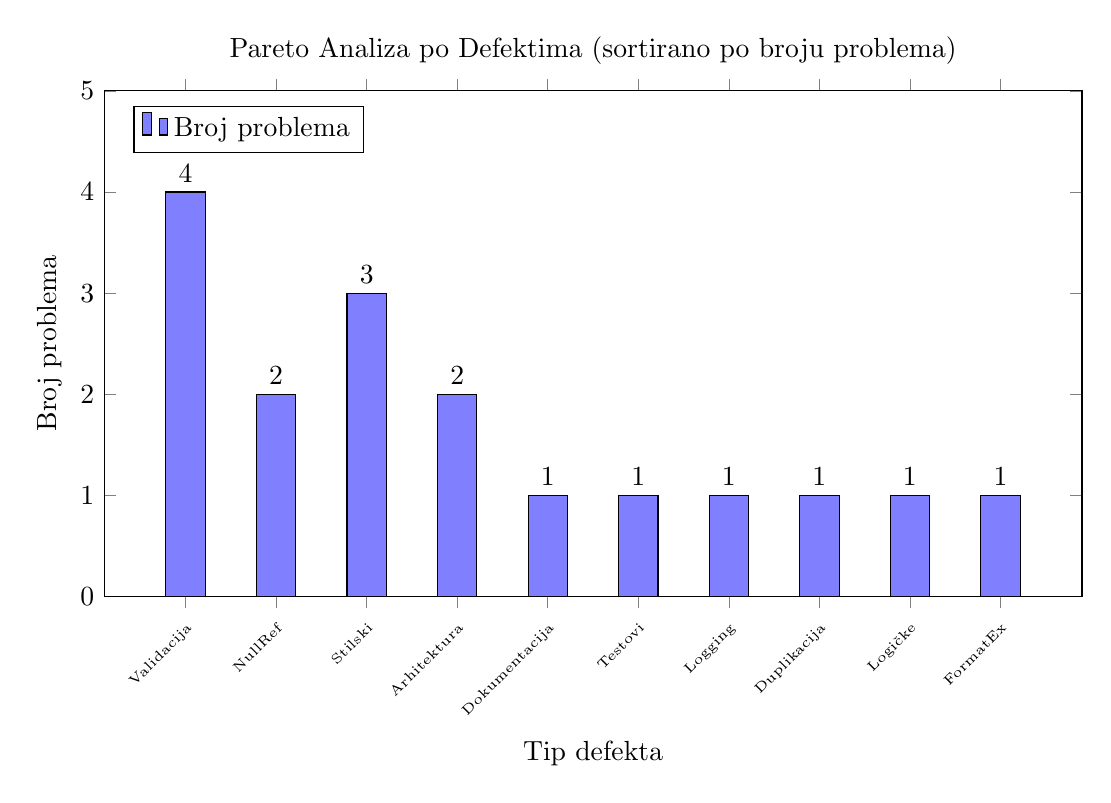
\begin{tikzpicture}
\begin{axis}[
    ybar,
    bar width=0.5cm,
    width=14cm,
    height=8cm,
    ylabel={Broj problema},
    xlabel={Tip defekta},
    symbolic x coords={Validacija, NullRef, Stilski, Arhitektura, Dokumentacija, Testovi, Logging, Duplikacija, Logičke, FormatEx},
    xtick=data,
    xticklabel style={rotate=45, anchor=north east, font=\tiny},
    ymin=0,
    ymax=5,
    legend pos=north west,
    title={Pareto Analiza po Defektima (sortirano po broju problema)},
    nodes near coords,
    nodes near coords align={vertical},
]
\addplot[fill=blue!50] coordinates {
    (Validacija, 4)
    (NullRef, 2)
    (Stilski, 3)
    (Arhitektura, 2)
    (Dokumentacija, 1)
    (Testovi, 1)
    (Logging, 1)
    (Duplikacija, 1)
    (Logičke, 1)
    (FormatEx, 1)
};
\legend{Broj problema}
\end{axis}
\end{tikzpicture}
\caption{Pareto dijagram - Analiza po defektima (sortirano po broju problema)}
\end{figure}

\begin{table}[H]
\centering
\begin{tabular}{lcc}
\toprule
\textbf{Tip Defekta} & \textbf{Broj} & \textbf{Kumulativni postotak} \\
\midrule
Validacija & 4 & 23.5\% \\
Stilski & 3 & 41.2\% \\
NullRef & 2 & 52.9\% \\
Arhitektura & 2 & 64.7\% \\
Dokumentacija & 1 & 70.6\% \\
Testovi & 1 & 76.5\% \\
Logging & 1 & 82.4\% \\
Duplikacija & 1 & 88.2\% \\
Logičke & 1 & 94.1\% \\
FormatEx & 1 & 100.0\% \\
\bottomrule
\end{tabular}
\caption{Kumulativna analiza po defektima}
\end{table}

\subsection{Analiza Prioriteta}

\begin{table}[H]
\centering
\begin{tabular}{lcc}
\toprule
\textbf{Prioritet} & \textbf{Broj Problema} & \textbf{Postotak} \\
\midrule
P1 (Kritično) & 4 & 26.7\% \\
P2 (Visoko) & 8 & 53.3\% \\
P3 (Srednje) & 2 & 13.3\% \\
P4 (Nisko) & 2 & 13.3\% \\
\bottomrule
\end{tabular}
\caption{Raspodjela problema po prioritetima}
\end{table}

\textit{Napomena: Ukupno 15 problema, ali neki problemi mogu imati više prioriteta.}

\textbf{Preporuke:}
\begin{itemize}
    \item \textbf{P1 (Kritično):} 4 problema - mora se riješiti odmah prije puštanja u produkciju
    \item \textbf{P2 (Visoko):} 8 problema - riješiti u narednom sprintu
    \item \textbf{P3 (Srednje):} 2 problema - riješiti kada bude vremena
    \item \textbf{P4 (Nisko):} 2 problema - riješiti kao cleanup
\end{itemize}

\section{Dobre Prakse}

Tokom inspekcije, identifikovane su i dobre prakse u kodu:

\begin{itemize}
    \item \textbf{Separation of Concerns:} Kod je dobro organizovan u modele i servise
    \item \textbf{Enum korištenje:} Dobro korištenje enuma za \texttt{Kategorija} i sortiranje
    \item \textbf{Korištenje LINQ:} Efektivno korištenje LINQ za filtriranje i pretraživanje
    \item \textbf{Try-catch blokovi:} Postoje try-catch blokovi u \texttt{Main} metodi
    \item \textbf{CultureInfo:} Korištenje \texttt{CultureInfo.InvariantCulture} za parsiranje brojeva
    \item \textbf{StringComparison:} Korištenje \texttt{StringComparison.OrdinalIgnoreCase} za case-insensitive poređenje
\end{itemize}

\section{Preporuke za Poboljšanje}

\subsection{Kratkoročne (Sprint 1)}

\begin{enumerate}
    \item Popraviti kritične greške (ISSUE-001, ISSUE-002, ISSUE-003)
    \item Dodati validaciju inputa na svim mjestima
    \item Ukloniti duplikaciju koda (ISSUE-004)
    \item Dodati osnovni logging
\end{enumerate}

\subsection{Srednjoročne (Sprint 2-3)}

\begin{enumerate}
    \item Dodati unit testove
    \item Integrirati dependency injection
    \item Dodati konfiguracijski fajl
    \item Standardizovati imenovanje
\end{enumerate}

\subsection{Dugoročne (Sprint 4+)}

\begin{enumerate}
    \item Dodati kompletnu dokumentaciju
    \item Implementirati CI/CD pipeline
    \item Dodati integracijske testove
    \item Razmotriti migraciju na web API ili desktop aplikaciju
\end{enumerate}

\section{Zaključak}

Aplikacija \textbf{RestaurantInventory} ima dobru osnovnu strukturu i separation of concerns, ali ima nekoliko kritičnih problema koji moraju biti riješeni prije produkcije. 

\textbf{Najveći problemi su:}
\begin{enumerate}
    \item \textbf{Kritične greške} koje mogu dovesti do crash-a aplikacije (NullReferenceException, FormatException, logičke greške)
    \item \textbf{Nedostaje validacija} na više mjesta što može dovesti do neočekivanog ponašanja
    \item \textbf{Nedostaju testovi i dokumentacija} što otežava održavanje i razvoj
\end{enumerate}

\textbf{Pareto analiza} pokazuje da se fokusiranjem na tri glavna uzroka (Validacija, Dokumentacija/Testiranje, Nekonzistentnost) može riješiti 66.7\% svih problema.

\textbf{Preporučeno je riješiti sve P1 i P2 probleme prije puštanja u produkciju.}

\section{Checklist za Pull Request}

\begin{itemize}
    \item[$\square$] Svi P1 problemi su riješeni
    \item[$\square$] Dodana je validacija na svim mjestima gdje se prima input
    \item[$\square$] Uklonjena je duplikacija koda
    \item[$\square$] Dodani su osnovni unit testovi
    \item[$\square$] Dodana je osnovna dokumentacija (README.md)
    \item[$\square$] Kod je prošao code review
    \item[$\square$] Nema compiler warnings
    \item[$\square$] Kod je formatiran prema standardima
\end{itemize}

\vspace{2cm}

\begin{center}
\rule{0.5\textwidth}{0.4pt}

\textbf{Kreirao:} [Ime Inspektora] \\
\textbf{Datum:} [Datum] \\
\textbf{Verzija izvještaja:} 1.0
\end{center}

\end{document}

